%\chapter{Introduction}
\section{Introduction}
This document describes an on-going project aimed for a
ROSE~\cite{roseWeb2008}-based end-to-end empirical tuning (also called
    autotuning) system. 
It is part of an SciDAC PERI~\cite{peri} project to enable performance
portability of DOE applications through an empirical tuning system.
Our goal is to incorporate a set of external tools interacting with
ROSE-based components to support the entire life-cycle of automated empirical optimization.
We strive to keep this document up-to-date for better communication among
project participants. 
This document is not meant to reflect the final design or implementation choices. 

% moved to later sections, Liao, 8/4/2009
%\begin{figure}[htbp]  
%	\centering
%		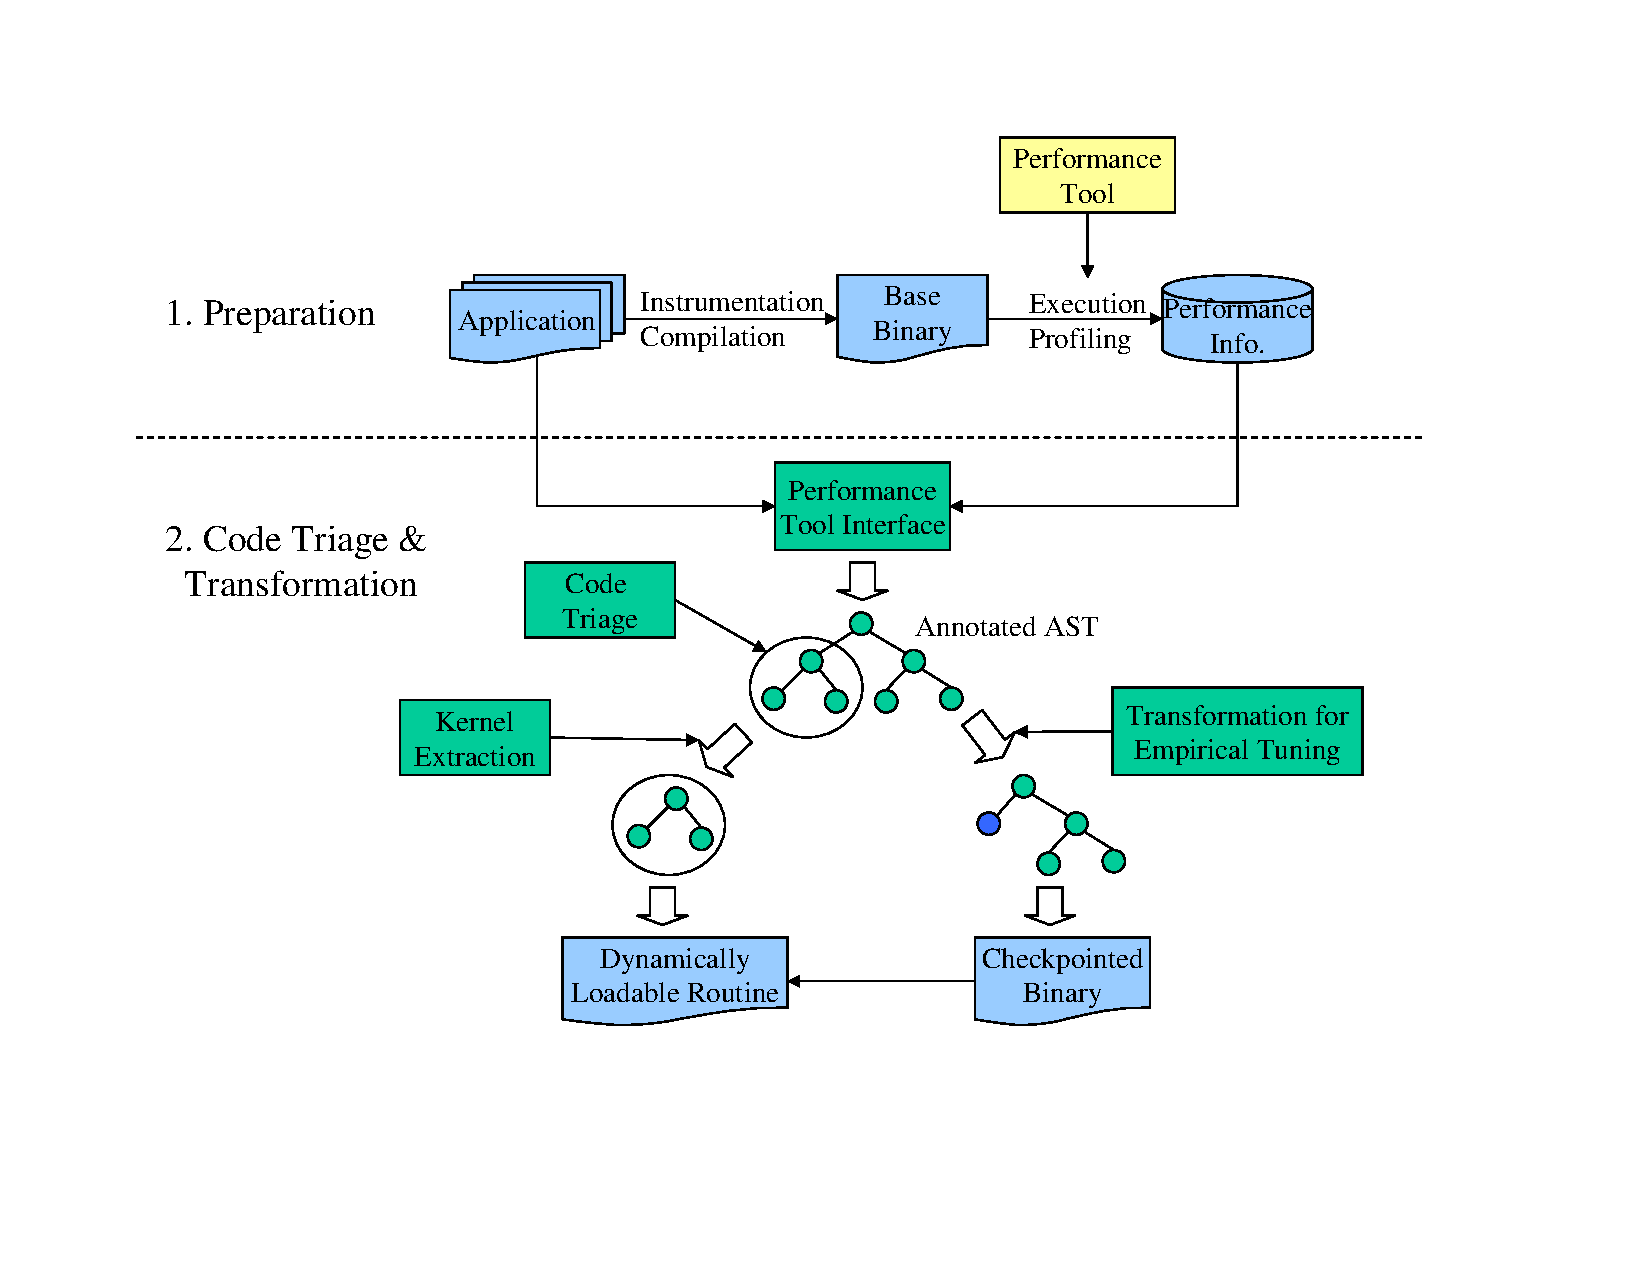
\includegraphics[width=1.2\textwidth]{phase12.pdf}
%	\caption{Phase 1 and 2 of the autotuning system}
%	\label{fig:phase12}
%\end{figure}
%
%\begin{figure}[htbp]  
%	\centering
%		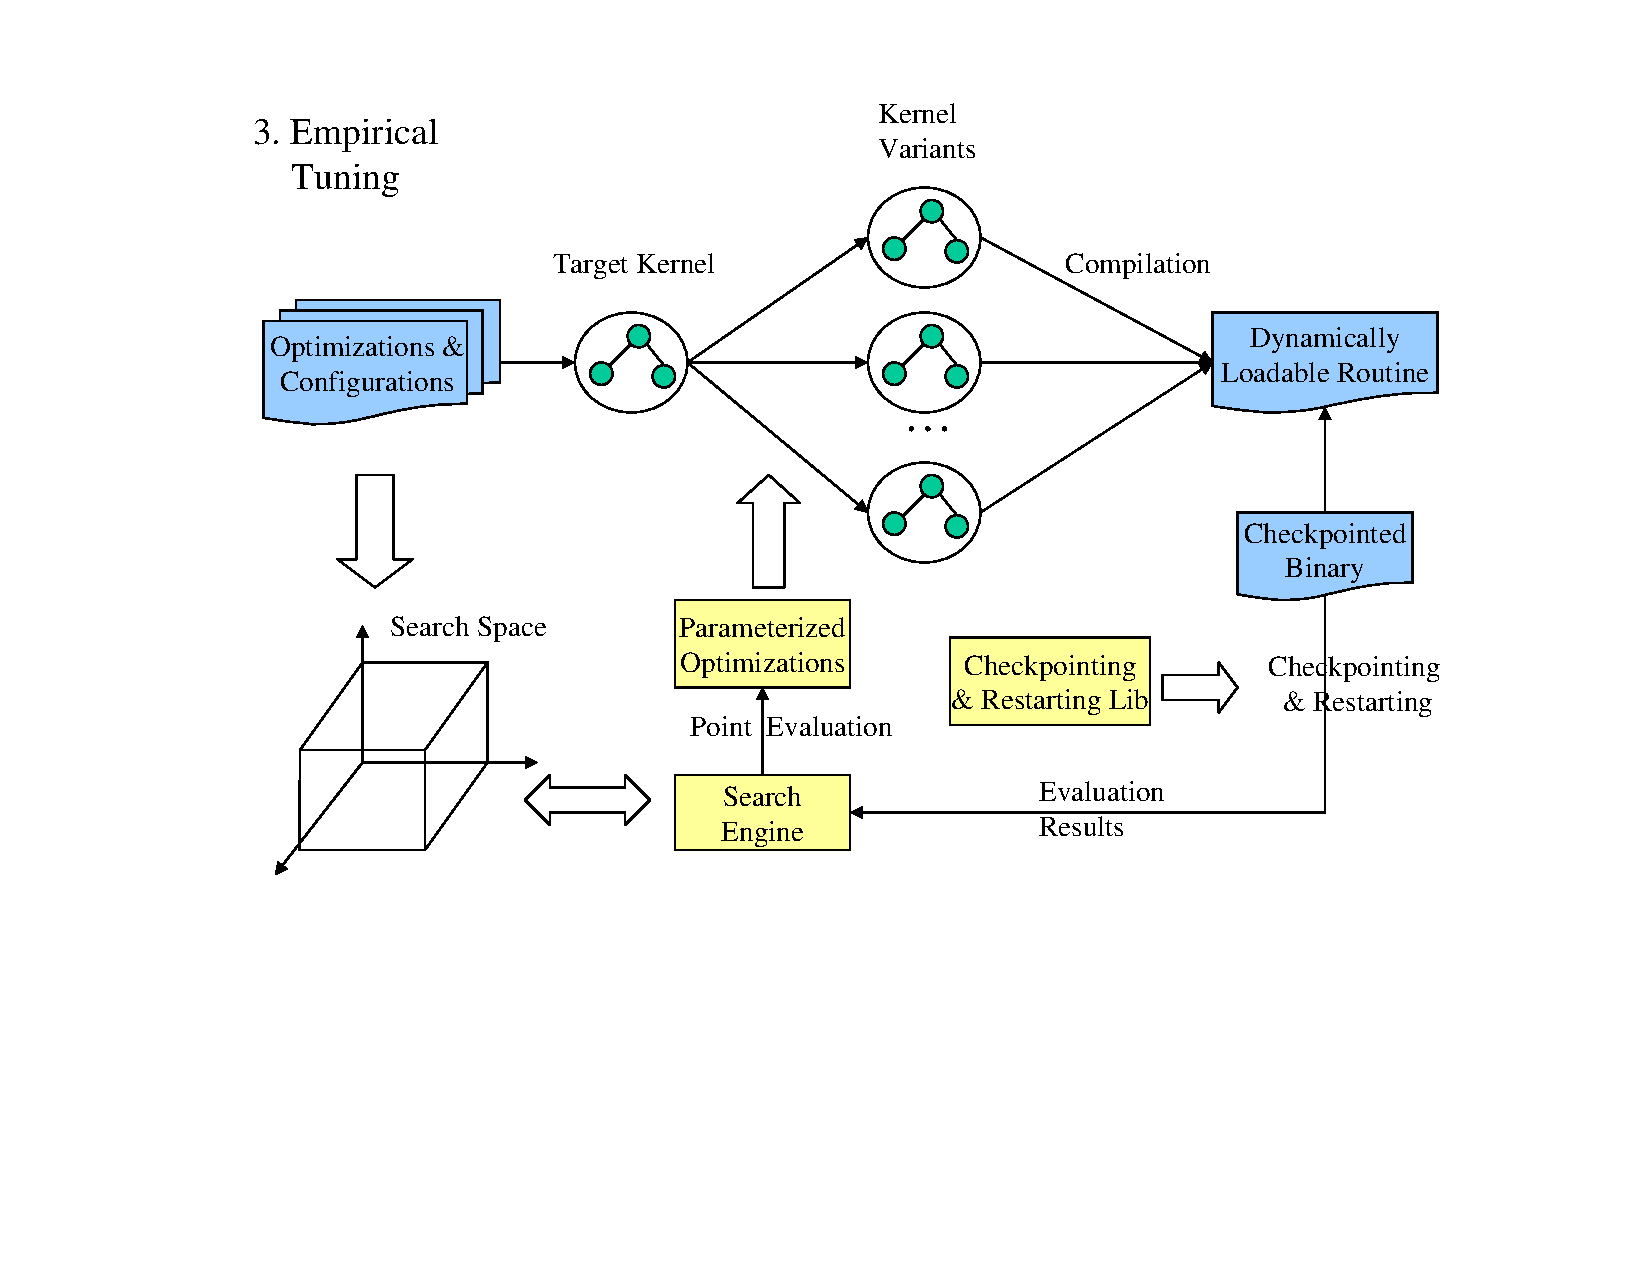
\includegraphics[width=1.2\textwidth]{phase3.pdf}
%	\caption{Phase 3 of the autotuning system}
%	\label{fig:phase3}
%\end{figure}

Currently, the ROSE-based autotuning system (shown in
    Fig.~\ref{fig:autotuning-overview}) is designed to work in three major
phases. 
%(Phase 1 and 2 are shown in Fig.~\ref{fig:phase12} and phase 3 is shown 
%in Fig.~\ref{fig:phase3}). 

\begin{figure}[htbp]  
                \vspace{-15ex}
	\centering
		\includegraphics[width=1.2\textwidth]{rose-autotuning-overview.pdf}
                \vspace{-15ex}
	\caption{A ROSE-based end-to-end autotuning system}
	\label{fig:autotuning-overview}
\end{figure}


\begin{enumerate}
% It starts with a preparation phase by using external performance tools to collect basic performance metrics of a target application. 
   \item {\bf Preparation} \\ 
      The preparation phase uses external performance tools to collect basic performance
      metrics of a target application. 

   \item {\bf Code triage, kernel extraction and transformations} \\
      This phase is carried out by a set of ROSE-based modules. 
      A ROSE tool interface
      module reads in both source files of the application and the performance data to
      construct an abstract syntax tree (AST) representation of the input code annotated
      with performance information. 

      Then a code triage module is followed to locate problematic targets (e.g
      loops) within the application. A set of potentially beneficial
      optimizations and/or their configurations for each target is chosen
      (manually for now) based on program analysis. 
% The remaining process is repeated for each target in order to find an
%optimal optimization solution. 

      After that, a ROSE AST Outliner extracts a selected target into
      a stand-alone kernel, which will in turn be compiled into a dynamically loadable library routine. 
      The application will be transformed accordingly and compiled to be a binary executable.
      This binary executable calls the outlined routine, collects performance metrics for
      the call.
      Optionally, a checkpointing/restarting library can be used to shorten
      the execution by stopping (checkpointing) and
      restarting immediately before calling the outlined function.

   \item {\bf Empirical tuning} \\
      The final phase does the actual empirical tuning. First of all, the
      potentially beneficial optimizations and their corresponding configurations
      are represented as points within an integral search space which can be handled by a search engine. 
      The search engine adopts some search policy to evaluate points in the search space
      and search for a point corresponding a transformation strategy leading to the best
      performance. 

      During this phase, multiple versions of the target kernel are generated by
      a parameterized translator%(e.g. a ROSE-based Loop Optimizer or other parameterized optimizers)
      from the searched points and compiled into dynamically loadable library
      routines. The performance of the kernel variants are measured one by one as the
      checkpointed binary is restarted multiple times and calls multiple versions
      of the dynamically loadable library routine. 
\end{enumerate}

We give some details about the system design and the current implementation
status in the following sections. 

A list of our current hardware/software configurations is given below:
\begin{itemize}
   \item A Dell Precision T5400 workstation with two sockets, each a 3.16
   GHz quad-core Intel Xeon X5460 processor, and total 8 GB memory; 
   \item Red Hat Enterprise Linux release 5.3 (Tikanga) Linux x86 kernel
   2.6.18-92.el5.perfctr SMP PREEMPT;
   \item PAPI 3.6.2;
   \item the Rice HPCToolkit version TRUNK-4.9.0=1280 (the latest
         release does not support the 32-bit machine we use, so we use an
         older version); 
   \item ROSE compiler version 0.9.4a, revision 6701 (providing a tool
       interface, outliner, loop translator, etc.);
   \item Berkeley Lab Checkpointing and Restarting library V. 0.8.2;
   \item POET from Univ. Texas San Antonio (We use its latest CVS version
         actually, not sure the exact release version number);
   \item the GCO search engine from Univ. of Tennessee (UTK) (We got a package from
         UTK directly, not sure the release number); 
%(Only an old version provided by UTK  works with the search engine right now).
   \item a C version jacobi iteration program, used as a simple example
   input code for autotuning.      

   \item the SMG2000~\cite{BrownSemicoarsening2000} (Semicoarsening Multigrid
         Solver) benchmark from the ASCI Purple, used as an example real
         application.
\end{itemize}


